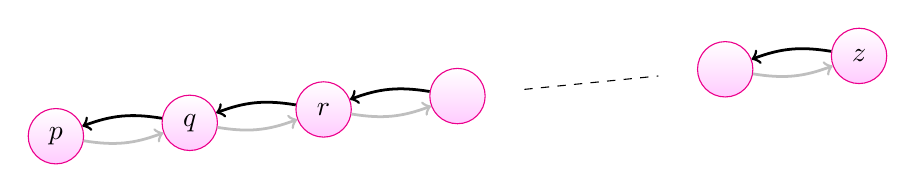
\begin{tikzpicture}[scale=.85]
\tikzset{nodo/.style={circle,minimum size=20pt,inner sep=0pt,draw, top color=white ,bottom color=magenta!20, magenta,text=black}}


  \draw (0,0) node[nodo](p) {$p$};
  \draw (2,.2) node[nodo] (q){$q$};  
  \draw (4,.4) node[nodo](r) {$r$};
  \draw (6,.6) node[nodo](x) {}; 
  \draw (10,1) node[nodo](y) {};
  \draw (12,1.2) node[nodo](k) {$z$};              

	\draw[->, line width=1pt] (k) to [bend right=15](y);
	\draw[->, gray!50, line width=1pt] (y)to[bend right=15] (k);   
    
    \draw[->, line width=1pt] (x) to [bend right=15](r);
	\draw[->, gray!50,line width=1pt] (r)to[bend right=15] (x);   
	
	\draw[->, line width=1pt] (r) to [bend right=15](q);
	\draw[->, gray!50,line width=1pt] (q)to[bend right=15] (r);   
	
	\draw[->, line width=1pt] (q) to [bend right=15](p);
	\draw[->, gray!50,line width=1pt] (p)to[bend right=15] (q);   
	
	\draw[dashed=5](7,0.7)--(9,0.9);
\end{tikzpicture}
